\section{Cuantificación y Codificación}

\begin{frame}
\frametitle{Cuantificación I}

\begin{figure}
  \centering
  \small
\scalebox{0.65}{
  \begin{psmatrix}[mnode=r,colsep=2.3,rowsep=0.1]
 [name=in]&[name=CAD]  \psframebox[fillstyle=solid,fillcolor=green,framesep=10pt,linecolor=gray,linewidth=0.4pt]{\parbox[c]{45ex}{\begin{psmatrix}[mnode=r,colsep=0.3,rowsep=0.1]
\psframebox[fillstyle=solid,fillcolor=white,framesep=10pt,linecolor=gray,linewidth=0.4pt]{\parbox[c]{10ex}{\centering Muestreador}} & \psframebox[fillstyle=solid,fillcolor=white,framesep=10pt,linecolor=gray,linewidth=0.4pt]{\parbox[c]{10ex}{\centering Cuantificador}} & \psframebox[fillstyle=solid,fillcolor=white,framesep=10pt,linecolor=gray,linewidth=0.4pt]{\parbox[c]{10ex}{\centering Codificador}}
 \end{psmatrix}
}}
& [name=out] \\
  & Conversión A/D
     
     % Connexions
     \visible<1->{\ncline[linecolor=lightgray]{->}{in}{CAD} \Bput{$x_a(t)$} \Aput{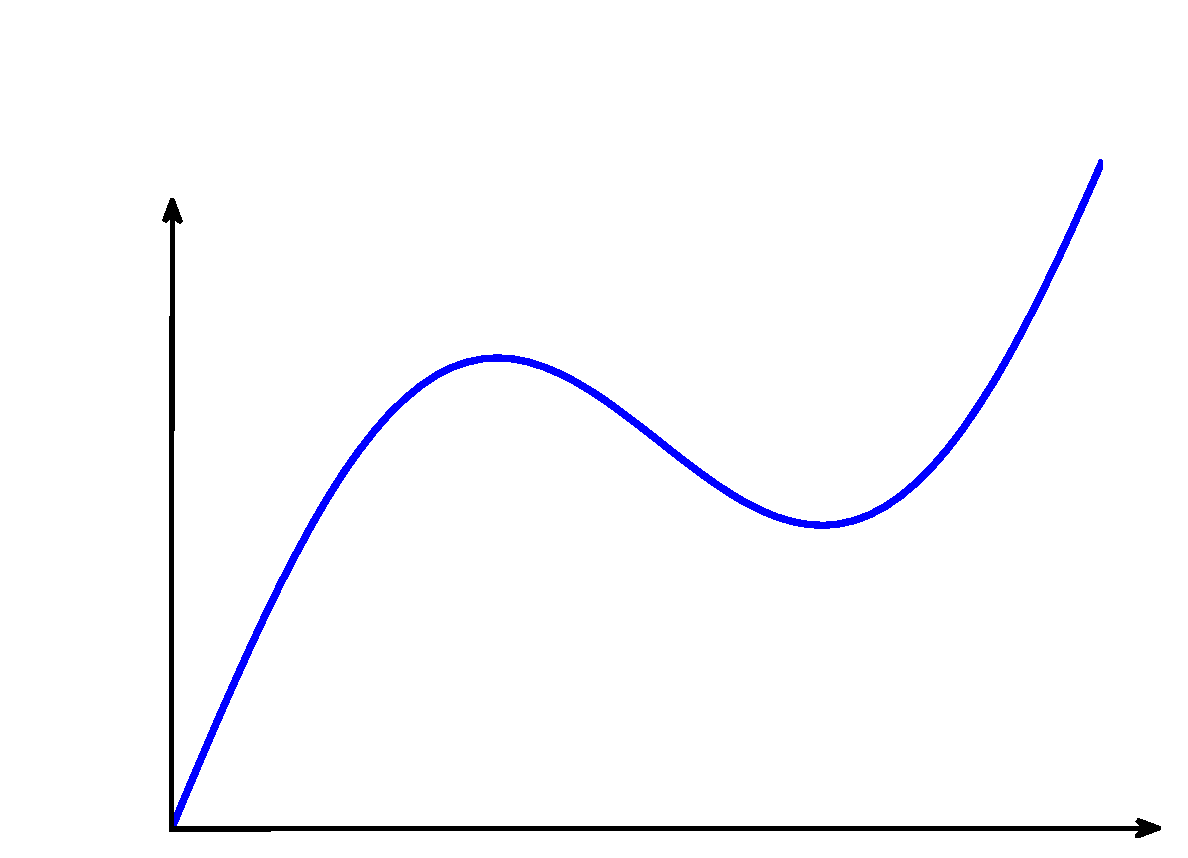
\includegraphics[width=1.5cm]{./Figures/input.eps} }} 
     \visible<1->{\ncline[linecolor=lightgray]{->}{CAD}{out} \Bput{$x_d(n)$} \Aput{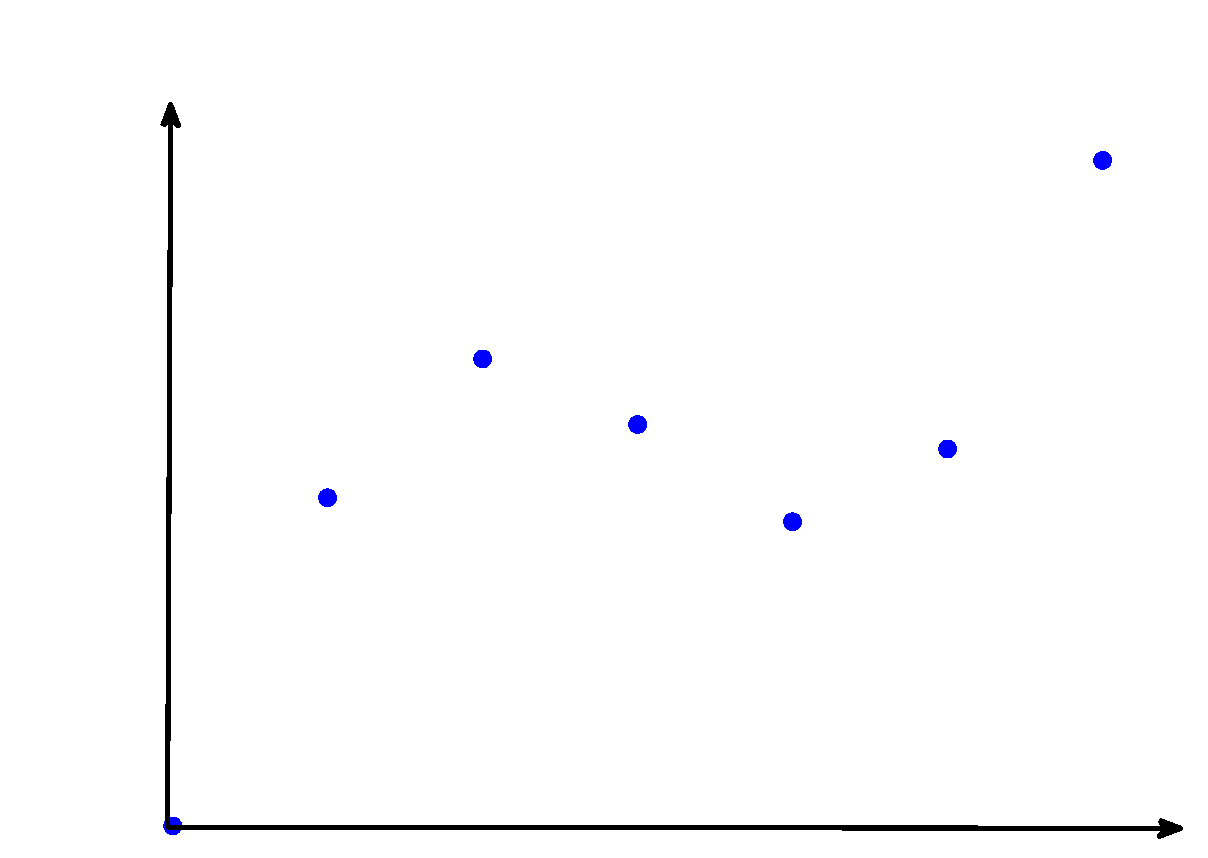
\includegraphics[width=1.5cm]{./Figures/inputD.eps} }} 
   
   \end{psmatrix}  
  }
\end{figure}

\vspace{-0.3cm}

\footnotesize
\begin{itemize}
\visible<2->{\item Una señal digital es una secuencia de números (muestras) en las que cada número se representa por un número finito de dígitos (precisión finita).}
\visible<3->{\item El proceso de convertir  una señal en tiempo discreto de amplitud constante (señal muestreada, $x(n)$) en una señal digital (doblemente discreta, $x_d(n)$) se denomina cuantificación:  \alert{ $x_d(n)=Q[x(n)]$}}
\visible<4->{\item Los niveles de cuantificación son los valores permitidos de la señal original.}
\visible<5->{\item El escalón de cuantificación o resolución $\Delta$ es  la distancia  entre dos niveles de cuantificación sucesivos.}
\begin{itemize}
\footnotesize
\visible<6->{\item El rango dinámico se define como el intervalo de valores $[x_{min},x_{max}]$ que toma la señal $x(n)$.}
\visible<7->{\item Si la señal $x(n) \in [x_{min},x_{max}]$ y existen $L$ niveles de cuantificación, $\Delta=\frac{x_{max}-x_{min}}{L-1}$.}
\visible<8->{\item Para un rango dinámico dado, si aumentamos el número de niveles aumenta la resolución (disminuye $\Delta$).}
\end{itemize} 		 
\end{itemize}

\end{frame}


\begin{frame}
\frametitle{Cuantificación II}

\footnotesize

\hspace{3cm}  \alert{ Cuantificación:  $x_d(n)=Q[x(n)]$}



\begin{itemize}
\item Tipos de cuantificación ($Q[\cdot]$):
\begin{itemize}
\footnotesize
\visible<2->{\item Redondeo: asigna cada muestra x(n) al valor del nivel de cuantificación más cercano.}
\visible<3->{\item Truncamiento: asigna cada muestra x(n) al valor del nivel de cuantificación inmediatamente inferior.}
\end{itemize}


\visible<4->{\item La diferencia entre la señal muestreada x(n) y la señal digital $x_d(n)$ se denomina error de cuantificación:  \alert{ $e_d(n)=x_d(n)-x(n)$}}

\visible<5->{\item La cuantificación es un proceso en el que se pierde información (hay un error) de forma irreversible, ya que se establece una relación entre muchos elementos (valores continuos de $x(n)$)) y uno único (nivel de cuantificación correspondiente).}


\visible<6->{\item Para un rango dinámico dado, si aumentamos el valor de niveles se reduce el error de cuantificación (ya que al disminuir $\Delta$ el error que se comete es más pequeño).}

\end{itemize}
\end{frame}

\begin{frame}
\frametitle{Ejemplo de cuantificación}

\footnotesize

\begin{itemize}
\color{olivegreen}
 \item Determinar la resoluci\'{o}n necesaria para cuantificar la señal $x(n)=0.9^n$ para representar exactamente los 10 primeros valores ($n \in [0,9]$).
 
 \visible<3->{
 \color{gray} Hay que ver cual de los x(n) necesita mayor número de dígitos: x(9) que necesita un total de 10 dígitos, por lo tanto tendríamos que cuantificarla con $\Delta=1E{-9}$}
 
 \color{olivegreen}
 \item ¿Cual es el error que se comete si se cuantifica la señal únicamente con dos dígitos?
 
 \visible<4->{
  \color{gray} Con dos dígitos, para el rango dinámico de valores del problema [0,1], tenemos que $\Delta=1E{-1}$.
  Se calcula el error como la diferencia entre el valor cuantizado (por truncamiento o redondeo) y el valor real.
 }
 \end{itemize}

\visible<2->{
 \color{gray}
\tiny
\hspace{1.5cm}\begin{tabular}{llcccc}
\hline 
 n & x(n) & $x_d(n)$ & $x_d(n)$  & $e_d(n)$  & $e_d(n)$\\
 & & Truncado & Redondeado & Truncado & Redondeado \\ \hline  
 0 &1.0   & 1.0 & 1.0  & 0.0 & 0.0\\  \hline
 1 &0.9   & 0.9 & 0.9 & 0.0 & 0.0\\  \hline
 2 &0.81 & 0.8 & 0.8  & -0.01 & -0.01 \\  \hline
 3 &0.729 & 0.7 & 0.7 & -0.029 & -0.029\\  \hline
 4 &0.6561 & 0.6 & 0.7 & -0.0561 &0.0439 \\  \hline
 5 &0.59049 & 0.5 & 0.6 & -0.09049 &0.00951\\  \hline
 6 &0.531441 & 0.5 & 0.5 & -0.031441 & -0.031441\\  \hline
 7&0.4782969 & 0.4 & 0.5 &-0.0782969 & 0.0217031\\  \hline
 8&0.43046721 & 0.4 &0.4 &-0.03046721& -0.03046721\\  \hline
 9 &0.387420489 & 0.3 &0.4 & -0.087420489 & 0.012579511\\  \hline

\end{tabular}
}

\end{frame}

%%%%%%%%%%%%%%%%%%%%%%%%%%%%%%%%%%%%%%%%%%%%%%%%%%%%%%%%%%%

\begin{frame}
\frametitle{Codificación}

\begin{figure}
  \centering
  \small
\scalebox{0.65}{
  \begin{psmatrix}[mnode=r,colsep=2.3,rowsep=0.1]
 [name=in]&[name=CAD]  \psframebox[fillstyle=solid,fillcolor=green,framesep=10pt,linecolor=gray,linewidth=0.4pt]{\parbox[c]{45ex}{\begin{psmatrix}[mnode=r,colsep=0.3,rowsep=0.1]
\psframebox[fillstyle=solid,fillcolor=white,framesep=10pt,linecolor=gray,linewidth=0.4pt]{\parbox[c]{10ex}{\centering Muestreador}} & \psframebox[fillstyle=solid,fillcolor=white,framesep=10pt,linecolor=gray,linewidth=0.4pt]{\parbox[c]{10ex}{\centering Cuantificador}} & \psframebox[fillstyle=solid,fillcolor=white,framesep=10pt,linecolor=gray,linewidth=0.4pt]{\parbox[c]{10ex}{\centering Codificador}}
 \end{psmatrix}
}}
& [name=out] \\
  & Conversión A/D
     
     % Connexions
     \visible<1->{\ncline[linecolor=lightgray]{->}{in}{CAD} \Bput{$x_a(t)$} \Aput{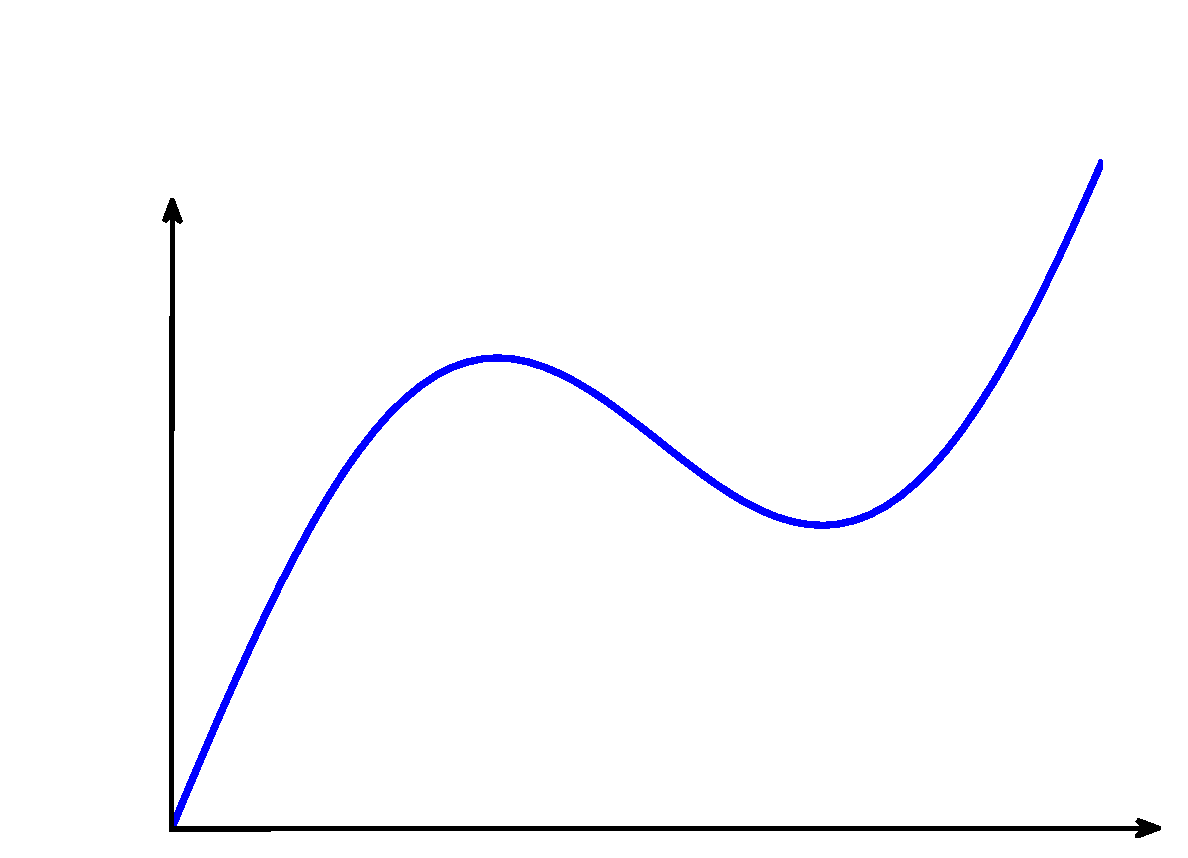
\includegraphics[width=1.5cm]{./Figures/input.eps} }} 
     \visible<1->{\ncline[linecolor=lightgray]{->}{CAD}{out} \Bput{$x_d(n)$} \Aput{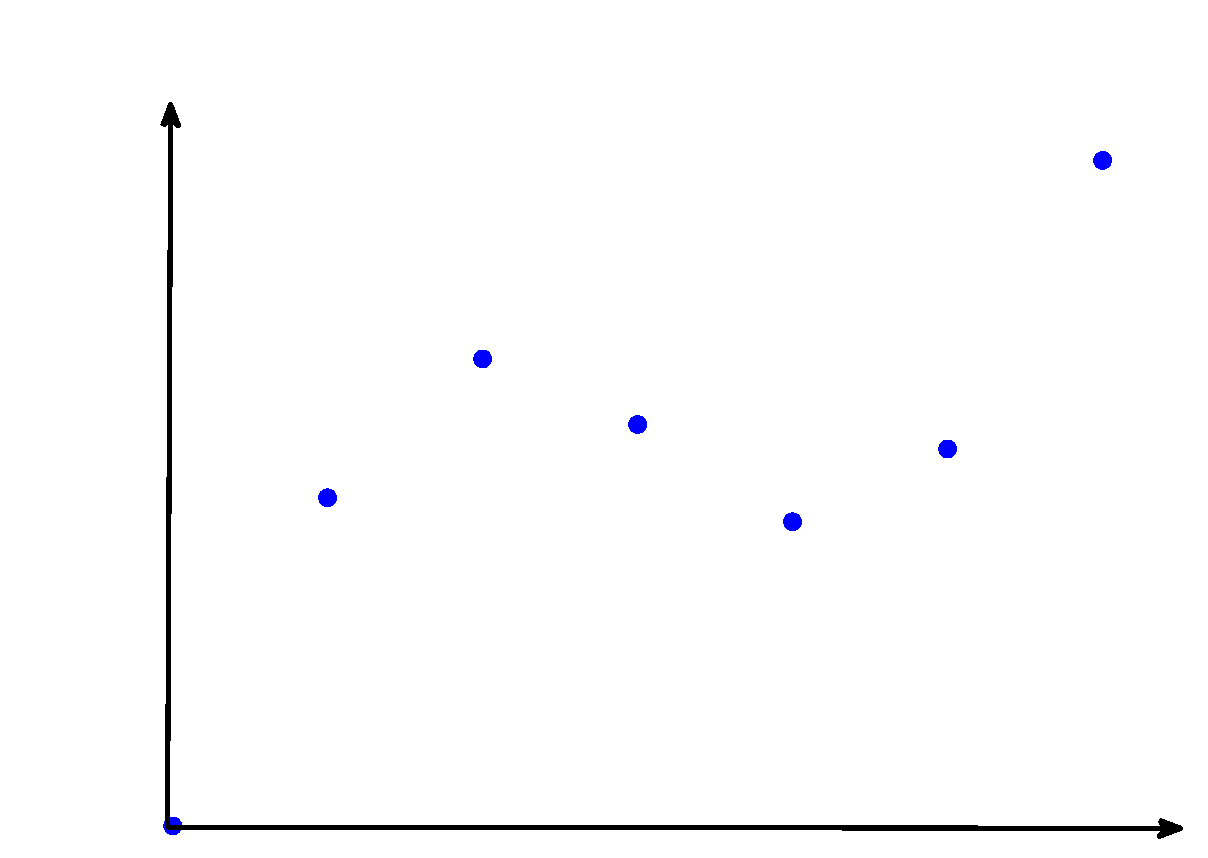
\includegraphics[width=1.5cm]{./Figures/inputD.eps} }} 
   
   \end{psmatrix}  
  }
\end{figure}

\vspace{-0.3cm}
\footnotesize

\begin{itemize}
\visible<1->{\item En el proceso de codificación se convierte la señal digital $x_d(n)$ en una cadena binaria $\{010101011\}$.}
\visible<2->{\item Si el número de niveles empleados para la cuantificación es $L$ se necesitan al menos $L$ niveles binarios  para representarla.}
\visible<3->{\item Una cadena binaria de $b$ bits permite representar $2^b$ números binarios diferentes.}
\visible<4->{\item Por lo tanto, $2^b \ge L \rightarrow b \ge log_2(L)$.

\item Es decir, el número de bits necesarios para codificar $L$ niveles es mayor o igual  $log_2(L)$.}

\vspace{0.2cm}
\visible<5->{
\hspace{-0.3cm}\color{olivegreen} Ejemplo: Calcular el número de bits necesarios para codificar 6 niveles de cuantificación.}

\visible<6->{
\color{gray}$L=6 \rightarrow log_2(L)= 2.585 \rightarrow b>=3$}


\end{itemize}


\end{frame}